% LaTeX Header for Bowen Island Biodiversity Data Atlas
% Created: 2025
% Author: Jay Matsushiba

% ============================================================================
% PACKAGES
% ============================================================================

% Page layout and margins
\usepackage[margin=1in, top=1in, bottom=1in, headsep=0.5in]{geometry}

% Font and text formatting
\usepackage[utf8]{inputenc}
\usepackage[T1]{fontenc}
\usepackage{helvet} % Helvetica (similar to Arial)
\renewcommand{\familydefault}{\sfdefault} % Use sans-serif as default

% Graphics and colors
\usepackage{graphicx}
\graphicspath{{./}{./images/}}
\usepackage{xcolor}
\definecolor{sfured}{RGB}{166,25,46}
\definecolor{bowengreen}{RGB}{76,129,58}
\usepackage{tikz}

% Headers and footers
\usepackage{fancyhdr}
\usepackage{lastpage}

% Tables and lists
\usepackage{booktabs}
\usepackage{longtable}
\usepackage{array}
\usepackage{enumitem}

% Links and references
\usepackage[hidelinks]{hyperref}
\usepackage{bookmark}

% Page numbers on every page including chapter pages
\usepackage{etoolbox}

% Caption formatting
\usepackage[font=small,labelfont=bf]{caption}

% ============================================================================
% PAGE STYLE
% ============================================================================

\pagestyle{fancy}
\fancyhf{} % Clear all header and footer fields

% Header setup - both logos on every page (respecting margins)
\fancyhead[L]{
\includegraphics[height=0.3in]{Bowen-Conservancy-Oval-Logo-6-green-text-transparent-background-400x112-1.png}}
\fancyhead[R]{
\includegraphics[height=0.3in]{SFU_horizontal_logo_rgb.png}}

% Footer setup - page numbers centered at bottom
\fancyfoot[C]{\thepage}

% Line thickness
\renewcommand{\headrulewidth}{0pt}
\renewcommand{\footrulewidth}{0pt}

% Apply to all page styles including chapter pages
\fancypagestyle{plain}{%
  \fancyhf{}
  \fancyhead[L]{
\includegraphics[height=0.3in]{Bowen-Conservancy-Oval-Logo-6-green-text-transparent-background-400x112-1.png}}
  \fancyhead[R]{
\includegraphics[height=0.3in]{SFU_horizontal_logo_rgb.png}}
  \fancyfoot[C]{\thepage}
  \renewcommand{\headrulewidth}{0pt}
  \renewcommand{\footrulewidth}{0pt}
}

% ============================================================================
% SECTION FORMATTING
% ============================================================================

\usepackage{titlesec}

% Chapter formatting - numbered chapters centered on own page (e.g., "1. Overview")
\titleformat{\chapter}[hang]
  {\vspace*{\fill}\normalfont\Huge\bfseries\color{bowengreen}}
  {\thechapter.}
  {1em}
  {}
  [\vspace*{\fill}\clearpage]

% Chapter spacing (left, before, after)
\titlespacing*{\chapter}{0pt}{0pt}{0pt}

% Section formatting
\titleformat{\section}
  {\normalfont\Large\bfseries\color{bowengreen}}
  {\thesection}
  {1em}
  {}

% Subsection formatting
\titleformat{\subsection}
  {\normalfont\large\bfseries\color{bowengreen}}
  {\thesubsection}
  {1em}
  {}

% ============================================================================
% TABLE OF CONTENTS FORMATTING
% ============================================================================

\usepackage{tocloft}

% TOC title formatting
\renewcommand{\cfttoctitlefont}{\Huge\bfseries\color{bowengreen}}

% % TOC spacing
% \setlength{\cftbeforechapskip}{10pt}
% \setlength{\cftbeforesecskip}{5pt}

% % Chapter formatting in TOC
% \renewcommand{\cftchapfont}{\bfseries}
% \renewcommand{\cftchappagefont}{\bfseries}

% ============================================================================
% CUSTOM COMMANDS
% ============================================================================

% % Map caption formatting
% \newcommand{\mapcaption}[1]{%
%   \begin{center}
%   \small\textit{#1}
%   \end{center}
% }

% % Species table formatting
% \newcommand{\speciesheader}{%
%   \toprule
%   \textbf{Species} & \textbf{Provincial} & \textbf{BC List} & \textbf{COSEWIC} & \textbf{IUCN} \\
%   \midrule
% }

% % Bold species names (for threatened/endangered)
% \newcommand{\boldspecies}[1]{\textbf{#1}}

% ============================================================================
% TITLE PAGE CUSTOMIZATION
% ============================================================================

\renewcommand{\maketitle}{%
  \begin{titlepage}
    \centering

    % Top logos
    \begin{minipage}{0.45\textwidth}
      
\includegraphics[width=0.8\textwidth]{Bowen-Conservancy-Oval-Logo-6-green-text-transparent-background-400x112-1.png}
    \end{minipage}
    \hfill
    \begin{minipage}{0.45\textwidth}
      \flushright
      
\includegraphics[width=0.6\textwidth]{SFU_horizontal_logo_rgb.png}
    \end{minipage}

    \vspace{2cm}

    % Title
    {\Huge\bfseries\color{bowengreen} DATA ATLAS\par}
    \vspace{0.5cm}
    {\Large\itshape In support of the development of a Bowen Island Biodiversity Plan\par}

    \vspace{0.5cm}

    % Cover image (optional - uncomment and provide image file if desired)
    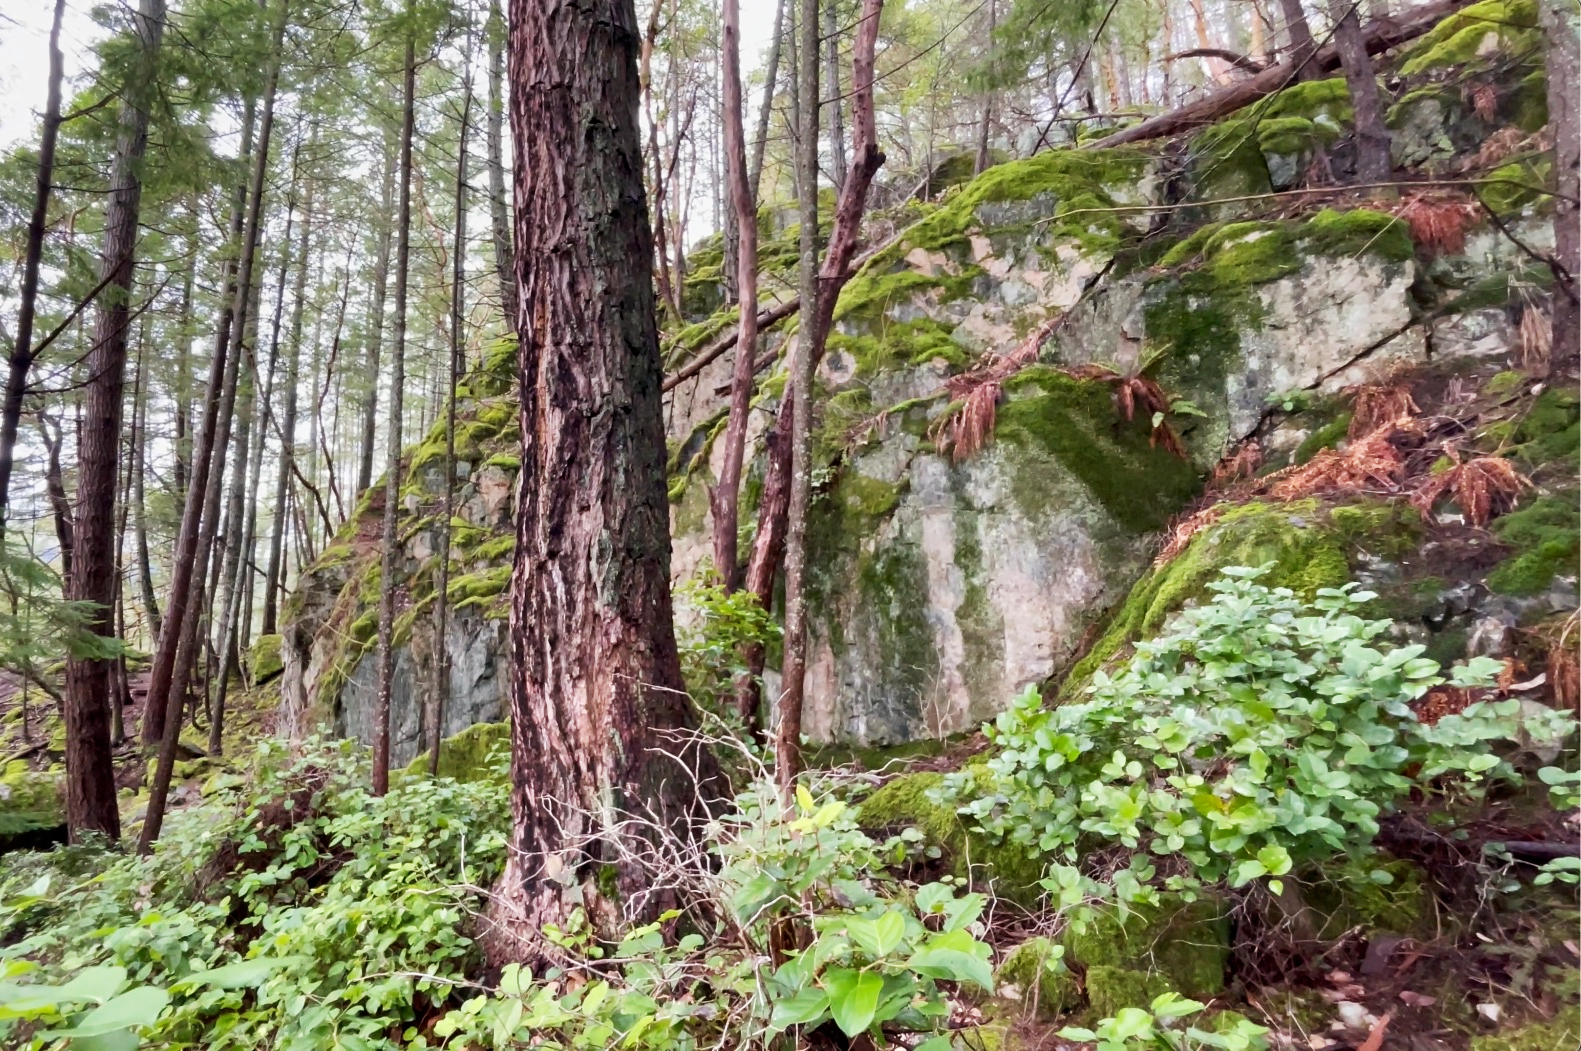
\includegraphics[width=\textwidth,height=1\textheight,keepaspectratio]{cover_image.png}

    \vfill

    % Authors
    {\large\bfseries Prepared by:\par}
    \vspace{0.2cm}
    {\large
    Jay Matsushiba, MSc\par
    \vspace{0.1cm}
    Wendy Palen, PhD\par
    \vspace{0.1cm}
    Tom Sisk, PhD\par
    }

    \vspace{1cm}

  \end{titlepage}
  \newpage
}

% ============================================================================
% DOCUMENT METADATA
% ============================================================================

\hypersetup{
  pdftitle={Bowen Island Biodiversity Data Atlas},
  pdfauthor={Jay Matsushiba, Wendy Palen, Tom Sisk},
  pdfsubject={Biodiversity Conservation Planning},
  pdfkeywords={Bowen Island, biodiversity, conservation, species distribution, habitat mapping},
  colorlinks=false,
  pdfborder={0 0 0}
}
